\documentclass{beamer}
\usepackage[utf8]{inputenc}
\usepackage[english,russian]{babel}
\usepackage{amsmath}
\usepackage{amsthm}
\usepackage{amssymb}
\usepackage{fancyhdr}
\usepackage{setspace}
\usepackage{graphicx}
\usepackage{colortbl}
\usepackage{tikz}
\usepackage{pgf}
\usepackage{subcaption}
\usepackage{listings}
\usepackage{indentfirst}
\usepackage{csquotes}
\usepackage{pgfpages}

\setbeamertemplate{navigation symbols}{}
%\setbeameroption{show notes on second screen}
\setbeamertemplate{note page}[plain]
\setbeamerfont{note page}{size=\tiny}

\mode<presentation> {
	\usetheme{Boadilla}
	\usecolortheme{lily}
}

\usefonttheme{serif}

\usepackage[sorting=nyt, backend=bibtex]{biblatex}
\addbibresource{bibliography.bib}

%----------------------------------------------------------------------------------------
%	TITLE PAGE
%----------------------------------------------------------------------------------------

\title[Prediction of Extremes]{Курсовая работа\\``Прогнозирование критических событий в моделях песчаной кучи БТВ и Манна''}

\author[Сапожников Денис]{
	Сапожников Денис Сергеевич БПМИ 192 \\
	\bigskip
	Руководитель КР: Шаповал Александр Борисович
}
\usepackage{datetime}
\newdate{date}{21}{06}{2022}
\date{\displaydate{date}}

\begin{document}

	\begin{frame}
		\titlepage

		\note{Добрый день, уважаемая комиссия. Меня зовут Сапожников Денис и сегодня я представляю Вам свою курсовую работу под названием Прогнозирование критических событий в моделях песчаной кучи БТВ и Манна”, которую я выполнял под научным руководством Шаповала Александра Борисовича.}
	\end{frame}

%------------------------------------------------


	\section{Введение}
%------------------------------------------------
	\begin{frame}{Модель песчаной кучи БТВ}
		\begin{onlyenv}<1>
			\begin{figure}[ht]
				\centering
				\begin{subfigure}{0.45\textwidth}
					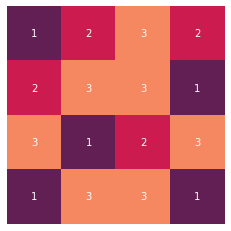
\includegraphics[width=\linewidth]{slides/btw_0}
				\end{subfigure}
				\begin{subfigure}{0.45\textwidth}
					\begin{itemize}
						\item Квадратная решетка $L \times L$
						\item В каждой клетке от $0$ до $3$ песчинок
						\item Каждую секунду добавляется одна песчинка в случайную клетку
					\end{itemize}
				\end{subfigure}
			\end{figure}
		\end{onlyenv}
		
		\begin{onlyenv}<2>
			\begin{figure}[ht]
				\centering
				\begin{subfigure}{0.45\textwidth}
					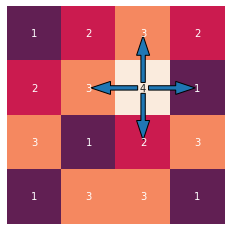
\includegraphics[width=\linewidth]{slides/btw_1}
				\end{subfigure}
				\begin{subfigure}{0.45\textwidth}
					Происходит обвал --- перераспределение песка (энергии)
				\end{subfigure}
			\end{figure}
		\end{onlyenv}
		
		\begin{onlyenv}<3>
			\begin{figure}[ht]
				\centering
				\begin{subfigure}{0.45\textwidth}
					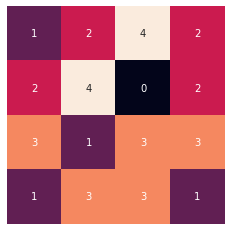
\includegraphics[width=\linewidth]{slides/btw_2}
				\end{subfigure}
				\begin{subfigure}{0.45\textwidth}
					Происходит обвал --- перераспределение песка
				\end{subfigure}
			\end{figure}
		\end{onlyenv}
	
		\begin{onlyenv}<4>
			\begin{figure}[ht]
				\centering
				\begin{subfigure}{0.45\textwidth}
					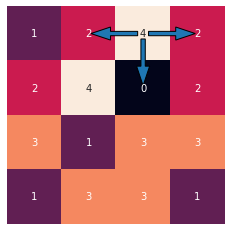
\includegraphics[width=\linewidth]{slides/btw_3}
				\end{subfigure}
				\begin{subfigure}{0.45\textwidth}
					Диссипация на границе
				\end{subfigure}
			\end{figure}
		\end{onlyenv}
	
		\begin{onlyenv}<5>
			\begin{figure}[ht]
				\centering
				\begin{subfigure}{0.45\textwidth}
					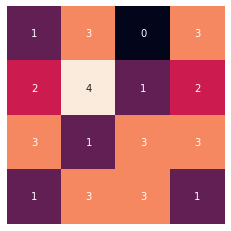
\includegraphics[width=\linewidth]{slides/btw_4}
				\end{subfigure}
				\begin{subfigure}{0.45\textwidth}
					Диссипация на границе
				\end{subfigure}
			\end{figure}
		\end{onlyenv}
		
		\begin{onlyenv}<6>
			\begin{figure}[ht]
				\centering
				\begin{subfigure}{0.45\textwidth}
					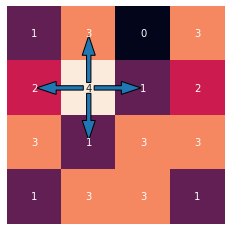
\includegraphics[width=\linewidth]{slides/btw_5}
				\end{subfigure}
				\begin{subfigure}{0.45\textwidth}
					Диссипация на границе
				\end{subfigure}
			\end{figure}
		\end{onlyenv}
	
		\begin{onlyenv}<7>
			\begin{figure}[ht]
				\centering
				\begin{subfigure}{0.45\textwidth}
					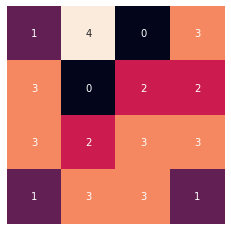
\includegraphics[width=\linewidth]{slides/btw_6}
				\end{subfigure}
				\begin{subfigure}{0.45\textwidth}
					Диссипация на границе
				\end{subfigure}
			\end{figure}
		\end{onlyenv}
	
		\begin{onlyenv}<8>
			\begin{figure}[ht]
				\centering
				\begin{subfigure}{0.45\textwidth}
					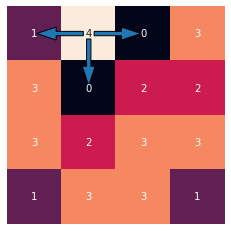
\includegraphics[width=\linewidth]{slides/btw_7}
				\end{subfigure}
				\begin{subfigure}{0.45\textwidth}
					Диссипация на границе
				\end{subfigure}
			\end{figure}
		\end{onlyenv}
	
		\begin{onlyenv}<9>
			\begin{figure}[ht]
				\centering
				\begin{subfigure}{0.45\textwidth}
					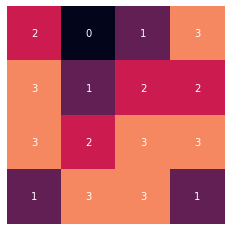
\includegraphics[width=\linewidth]{slides/btw_8}
				\end{subfigure}
				\begin{subfigure}{0.45\textwidth}
					\begin{enumerate}
						\item Размер события --- это количество обвалов до стабилизации
						\item Долгое накопление энергии и её мгновенное перераспределение
					\end{enumerate}
				\end{subfigure}
			\end{figure}
		\end{onlyenv}
	\end{frame}

	\begin{frame}{Обзор литературы}
		\begin{itemize}
			\item<1-> Появление модели песчаной кучи и теории самоорганизованных систем оказало вклад в развитие целых областей: стат. физика, экнономика, нейробиология и других
			\item<2-> Наблюдение степенного закона
			\only<2-2>{
				\begin{figure}[h]
					\centering
					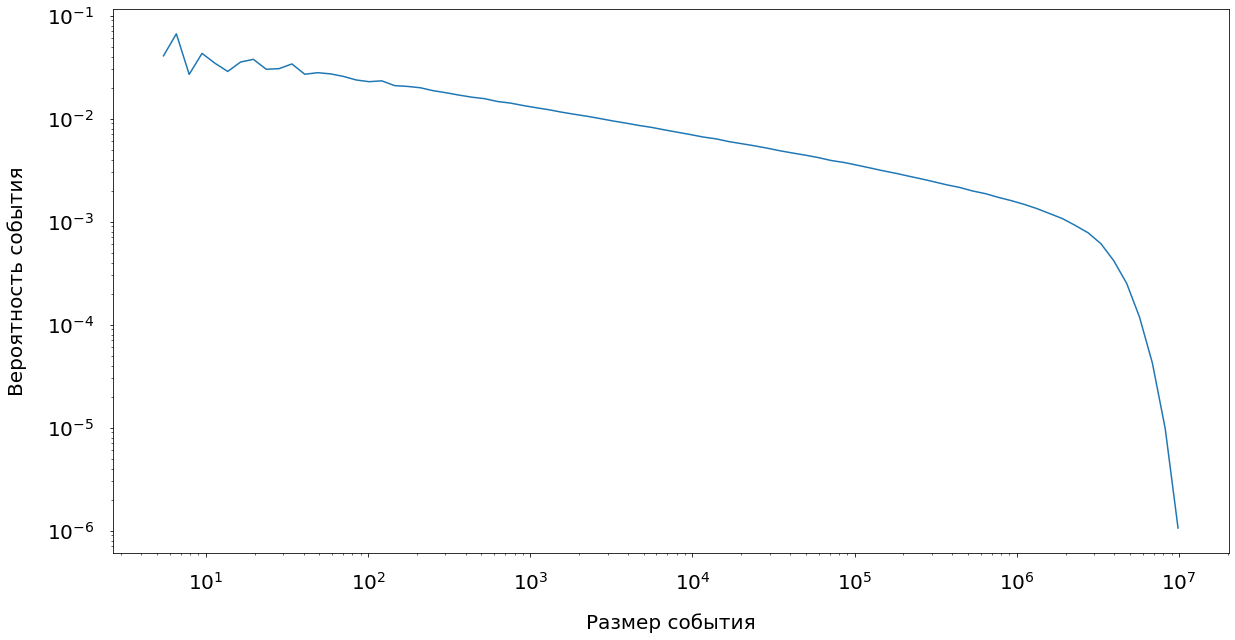
\includegraphics[width=0.8\linewidth]{slides/power_law}
					\caption*{Плотность распределения размеров событий в модели БТВ для решётки размера $L=64$}
				\end{figure}
			}
			\item<3-> Существует множество разных моделей песчаной кучи, которые можно получить заменой правил обвала и геометрии решетки
			\item<4-> В классе симметричных правил обвала на квадратной решетке существует лишь одна альтернативная модель относительно модели БТВ --- модель Манна, или стохастическая модель
			\item<5-> Наличие степенного закона --- индикатор отсутствия прогнозирования крупных событий
			\item<6-> Попытки прогнозирования представлены в работах Hallerberg~(2009), Delucia~(2015)
		\end{itemize}


		\note{}
	\end{frame}

	\section{Постановка задачи}

	\begin{frame}{Постановка задачи}
		\begin{itemize}
			\item<1-> Провести сравнительный анализ прогнозируемости крупных событий в моделях БТВ и Манна для конкретных конечных систем и термодинамического предела
			\item<2-> Найти скейлинг эффективности прогноза относительно объёма системы
			\item<3-> Соотнести скейлинг эффективности прогноза со скейлингом степенного распределения событий по размерам для конечной системы
		\end{itemize}

		\note{}
	\end{frame}

	\begin{frame}{Метрики}
		\begin{itemize}
			\item<1-> Качество прогноза $\varepsilon$ измеряется с помощью ROC-кривых
			\begin{figure}[h]
				\centering
				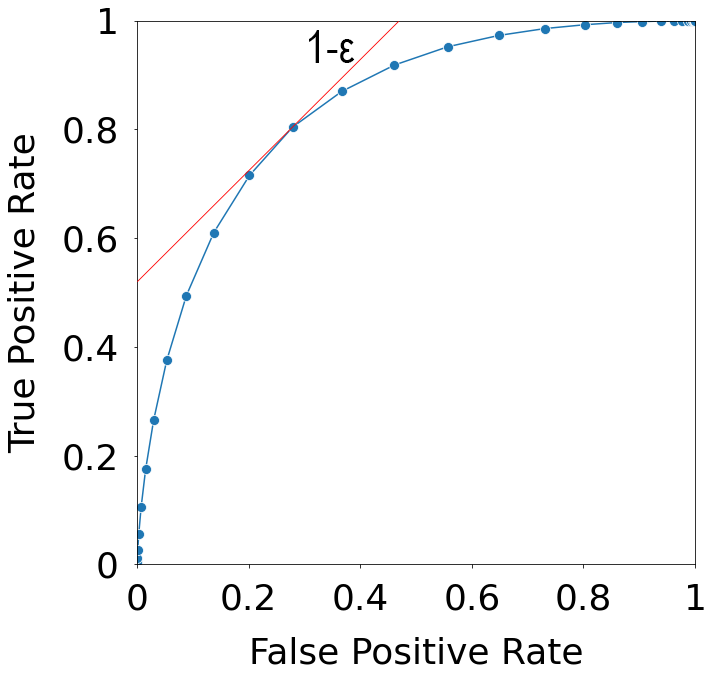
\includegraphics[width=0.5\linewidth]{slides/roc_curve_eps}
			\end{figure}
		\end{itemize}
	\end{frame}

	\begin{frame}{Алгоритм прогноза}
		\begin{enumerate}
			\item Пусть $\{s_n\}_{i=1}^{N}$ --- выборка из размеров событий. Она разбивается пополам на тренировочную и тестовые части
			\item Предсказываем вероятность крупных события $X_i = I[s_i > \eta]$
			\item Вычисляется переменная принятия решения
			
			$$ y_i = \sum\limits_{k=1}^{i} a^k \cdot s_{i-k} $$
			
			\item Вычисляется совместное распределение на тренировочной выборке $P(X,y)$
			\item По совместному распределению делаются прогнозы на тестовой выборке
		\end{enumerate}
	\end{frame}

	\begin{frame}{Качество прогноза}
		\begin{onlyenv}<1-1>
		\begin{figure}[h]
			\centering
			\begin{subfigure}[t]{0.45\textwidth}
				\centering
				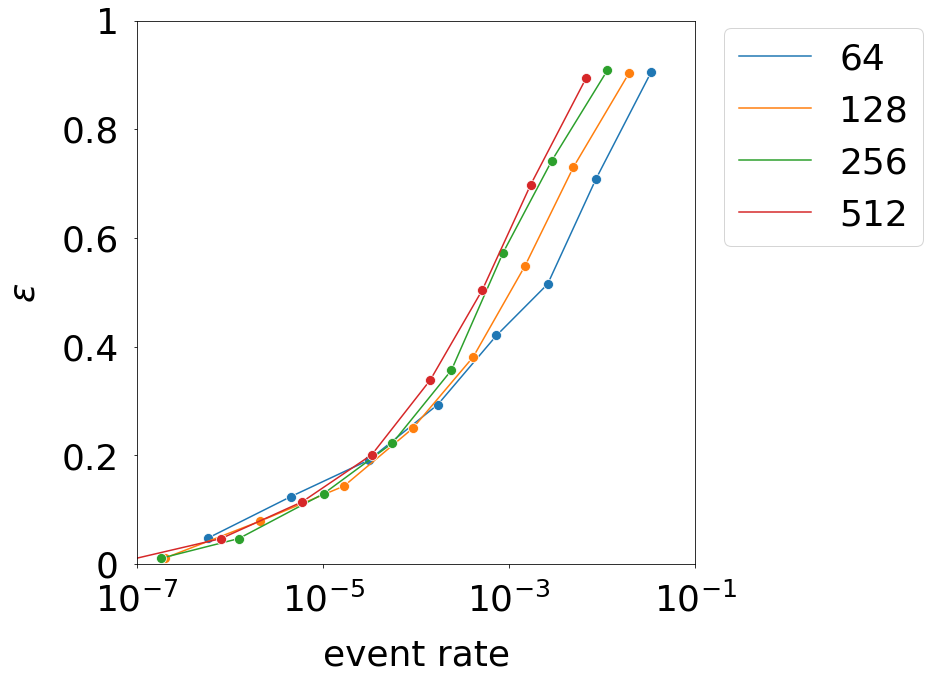
\includegraphics[width=\textwidth]{images/eps_vs_event_rate_manna}
				\caption{Модель Манна}
				\label{pic:event_rate_manna}
			\end{subfigure}
			\begin{subfigure}[t]{0.45\textwidth}
				\centering
				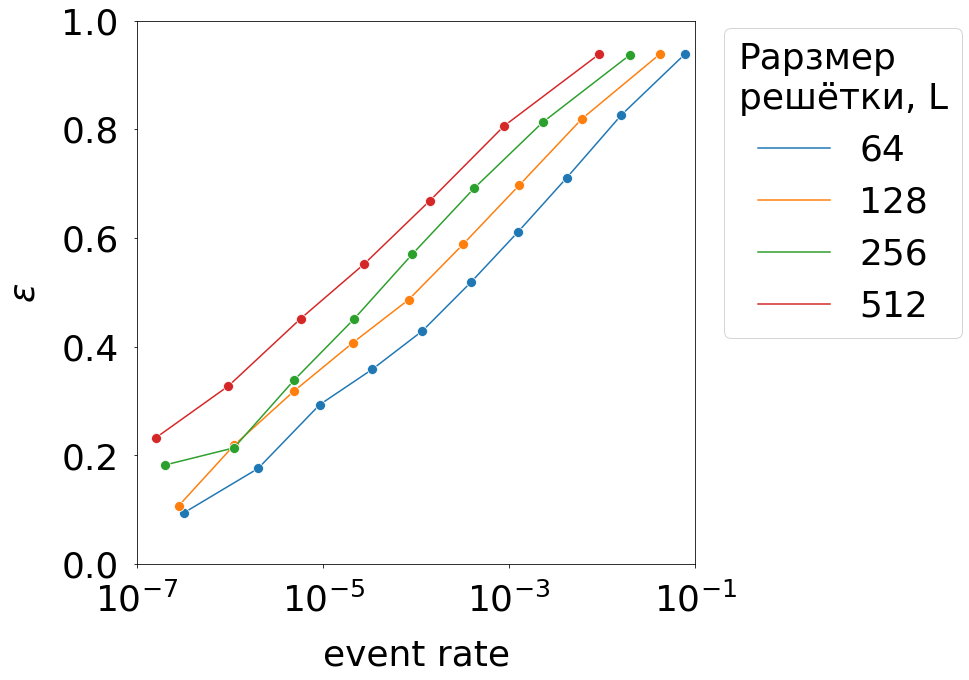
\includegraphics[width=\textwidth]{images/eps_vs_event_rate_btw}
				\caption{Модель БТВ}
				\label{pic:event_rate_btw}
			\end{subfigure}
			\caption*{Качество прогноза $\varepsilon$ в зависимости от частоты встречаемости событий $event\ rate$}\label{pic:event_rate}
		\end{figure}
		\end{onlyenv}
	
		\begin{onlyenv}<2-2>
			\begin{figure}[h]
				\centering
				\begin{subfigure}[t]{0.45\textwidth}
					\centering
					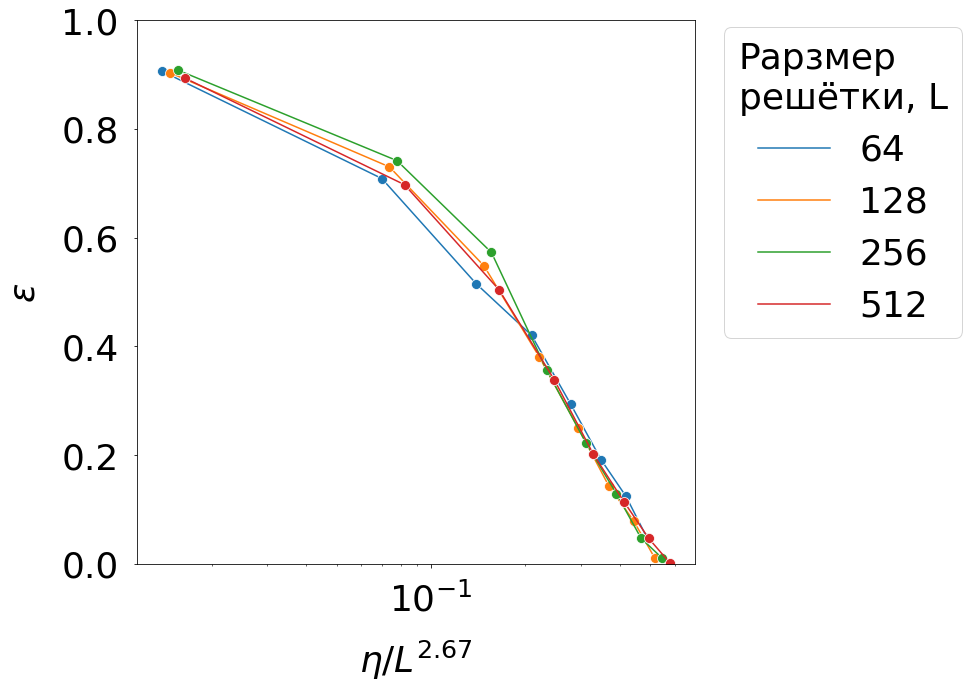
\includegraphics[width=\textwidth]{images/manna_eps_vs_eta}
					\caption{Модель Манна}
				\end{subfigure}
				\begin{subfigure}[t]{0.45\textwidth}
					\centering
					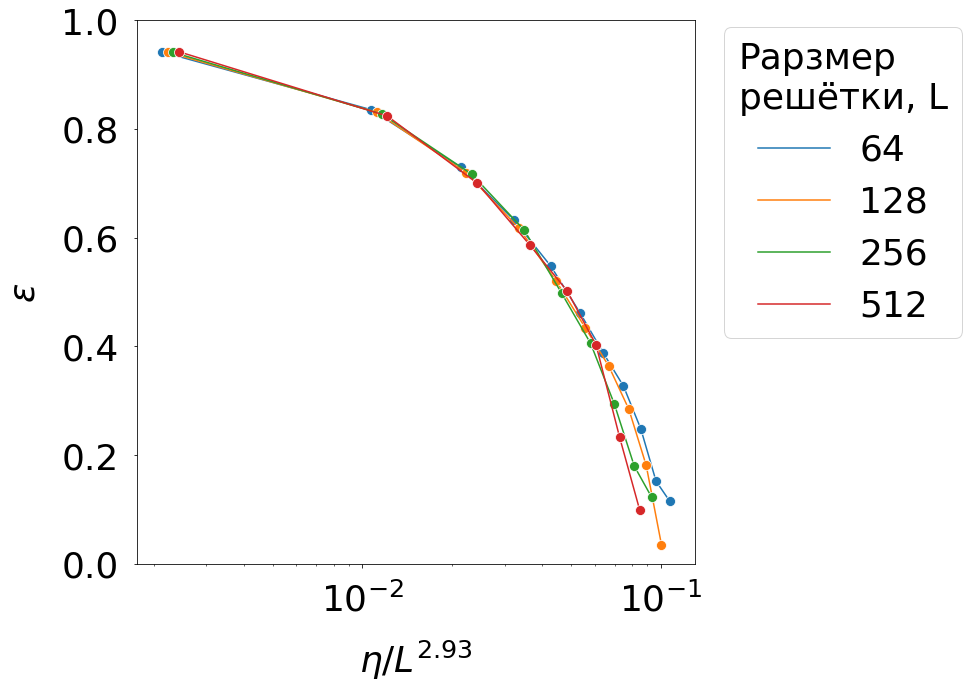
\includegraphics[width=\textwidth]{images/btw_eps_vs_eta}
					\caption{Модель БТВ}
				\end{subfigure}
				\caption*{Качество прогноза $\varepsilon$ в зависимости от нормированного размера крупного события $\eta/L^{\gamma}$}
			\end{figure}
		\end{onlyenv}
		
		\note{}
	\end{frame}

	\begin{frame}{Результаты}
		\begin{itemize}
			\item<1-> В модели Манна качество прогноза не зависит от объёма системы
			\item<2-> В модели БТВ качество прогноза падает с ростом объёма системы
			\item<3-> Скейлинг эффективности прогноза в модели Манна совпадает со скейлингом плотности распределений событий, а в модели БТВ -- со скейлингом крупнейшего события
			\item<4-> Модель песчаной кучи обладает большой памятью
		\end{itemize}

		\note{}
	\end{frame}

	%\begin{frame}
	%	\printbibliography
	%\end{frame}
	
	\begin{frame}{Шкалирование плотности распределения}
		\begin{onlyenv}<1>
			\begin{figure}[h]
				\centering
				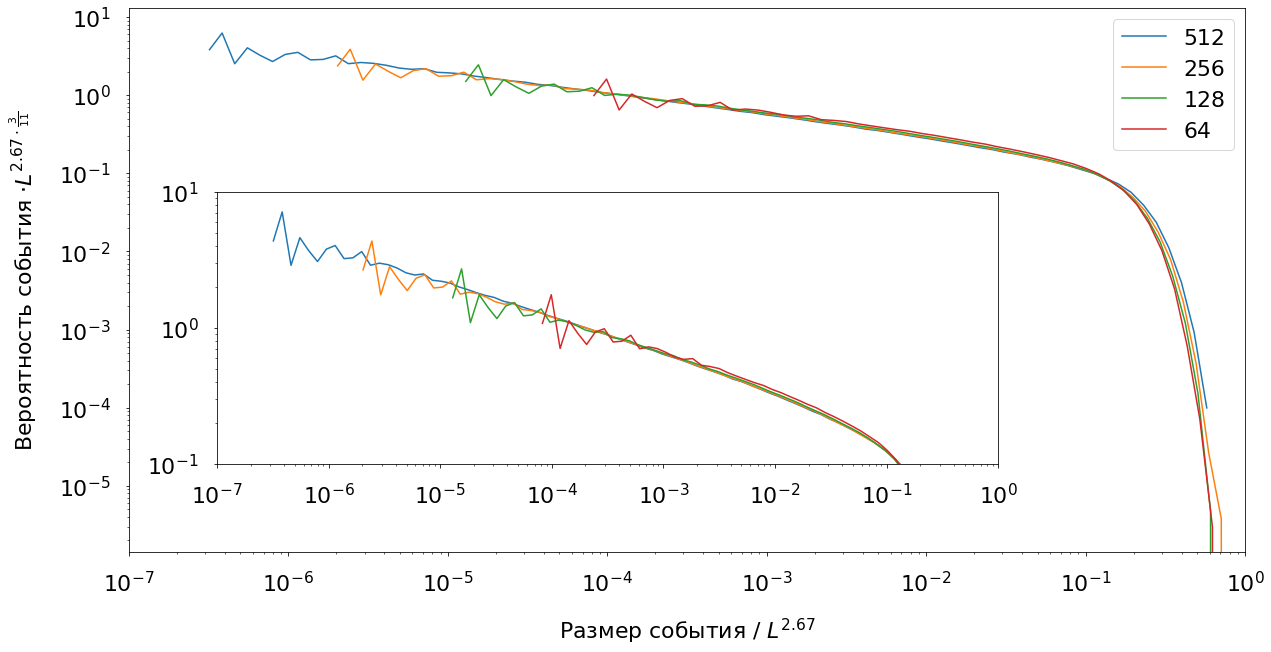
\includegraphics[width=\textwidth]{images/manna_distribution_267}
				\caption*{Шкалирование плотности распределения в модели Манна, $\tau = 2.67$}
			\end{figure}
		\end{onlyenv}
		
		\begin{onlyenv}<2>
			\begin{figure}[h]
				\centering
				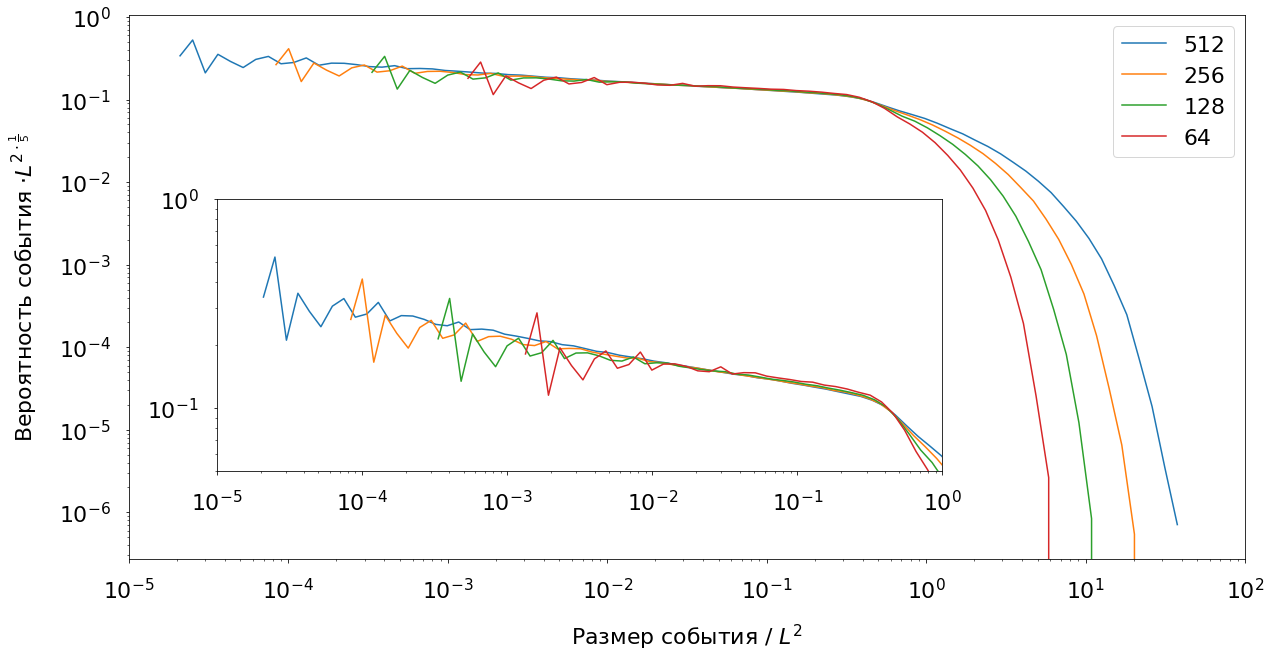
\includegraphics[width=\textwidth]{images/btw_distribution_200}
				\caption*{Шкалирование плотности распределения в модели БТВ, $\tau = 2$}
			\end{figure}
		\end{onlyenv}
	
		\begin{onlyenv}<3>
			\begin{figure}[h]
				\centering
				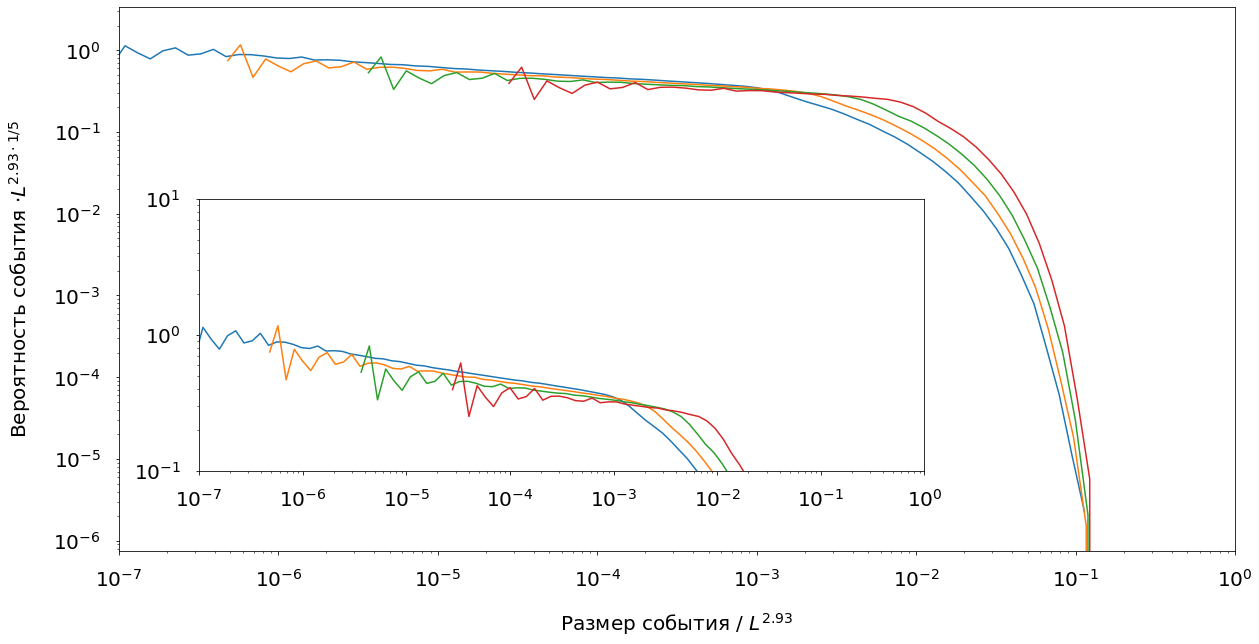
\includegraphics[width=\textwidth]{images/btw_distribution_293}
				\caption*{Шкалирование плотности распределения в модели БТВ, $\tau = 2.93$}
			\end{figure}
		\end{onlyenv}
	\end{frame}

	\begin{frame}{Влияние гиперпарматра $a$}
		\begin{figure}[h]
			\centering
			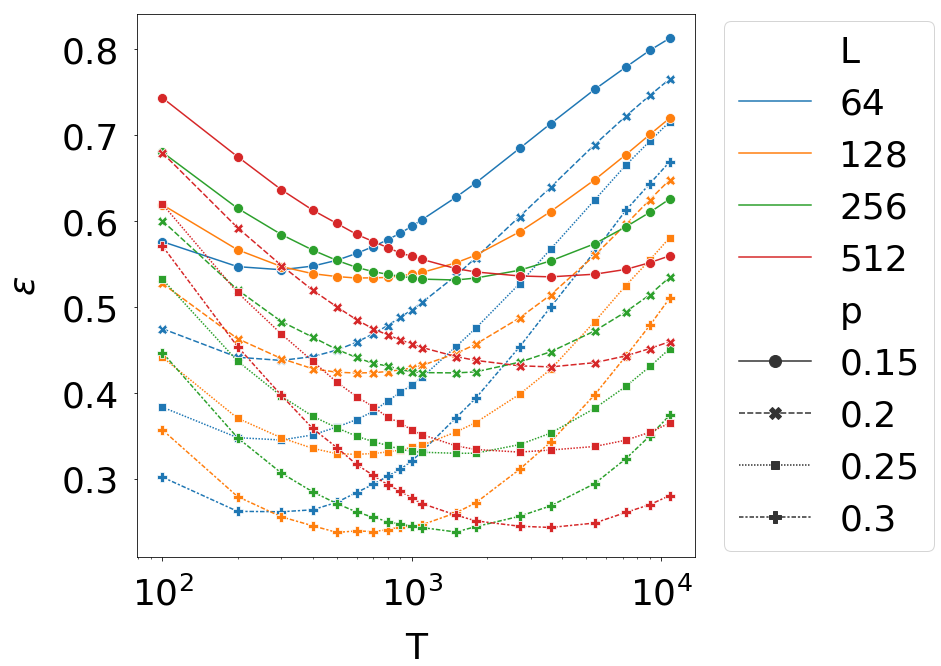
\includegraphics[width=0.8\textwidth]{images/manna_t_267}
			\caption*{Зависимость качества прогноза $\varepsilon$ от гиперпараметра $a$, переведенного в логарифмическую шкалу: $a = \exp(-T)$}
		\end{figure}
	\end{frame}

	\begin{frame}{О скейлинге эффективности прогноза}
		\begin{onlyenv}<1>
			\begin{figure}[h]
				\centering
				\centering
				\hspace{-15mm}
				\begin{subfigure}[t]{0.27\textwidth}
					\centering
					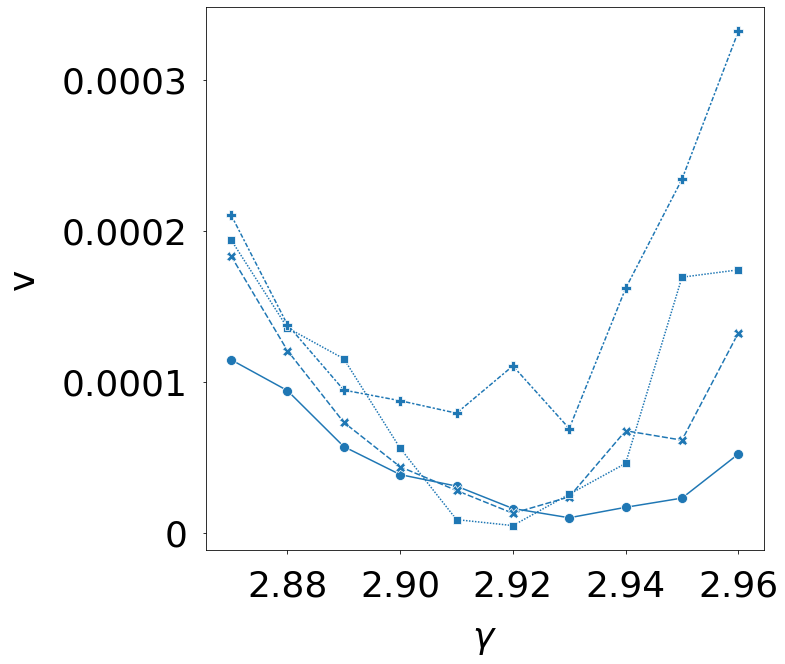
\includegraphics[height=\textwidth]{images/var_btw}
					\caption{Дисперсия}
				\end{subfigure}
				\hspace{5mm}
				\begin{subfigure}[t]{0.27\textwidth}
					\centering
					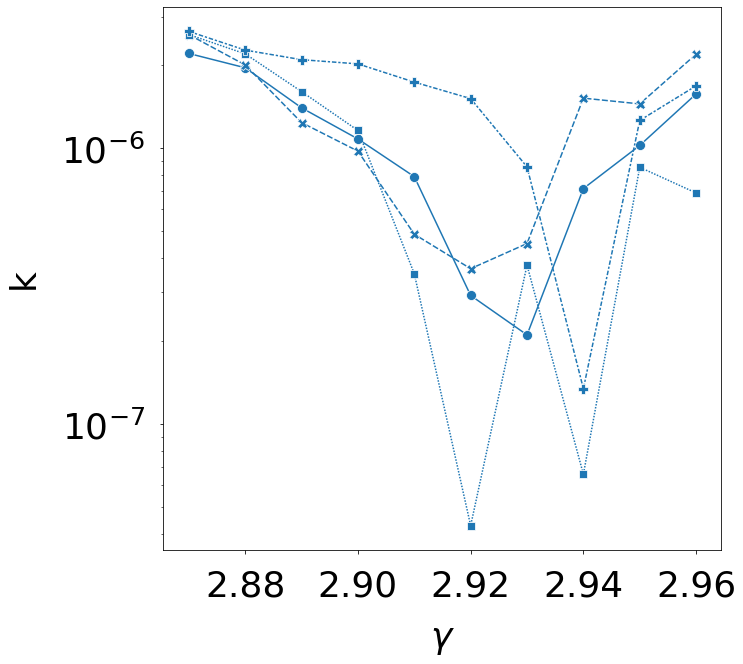
\includegraphics[height=\textwidth]{images/k_btw}
					\caption{Абсолютное значение коэффициента регрессирующей прямой}
				\end{subfigure}
				\hspace{0mm}
				\begin{subfigure}[t]{0.27\textwidth}
					\centering
					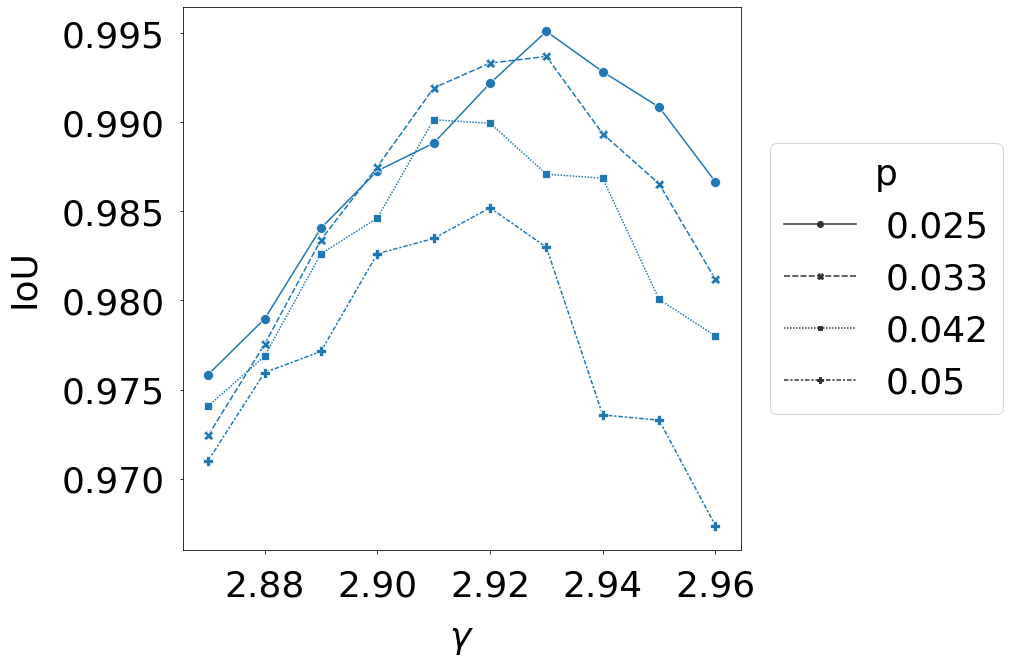
\includegraphics[height=\textwidth]{images/IoU_btw}
					\caption{IoU}
				\end{subfigure}
				\caption*{Метрики качества шкалирования в модели БТВ в зависимости от параметра $\gamma$}\label{pic:btw_scaling_metrics}
			\end{figure}
		\end{onlyenv}
		
		\begin{onlyenv}<2>
			\begin{figure}[h]
				\centering
				\hspace{-15mm}
				\begin{subfigure}[t]{0.27\textwidth}
					\centering
					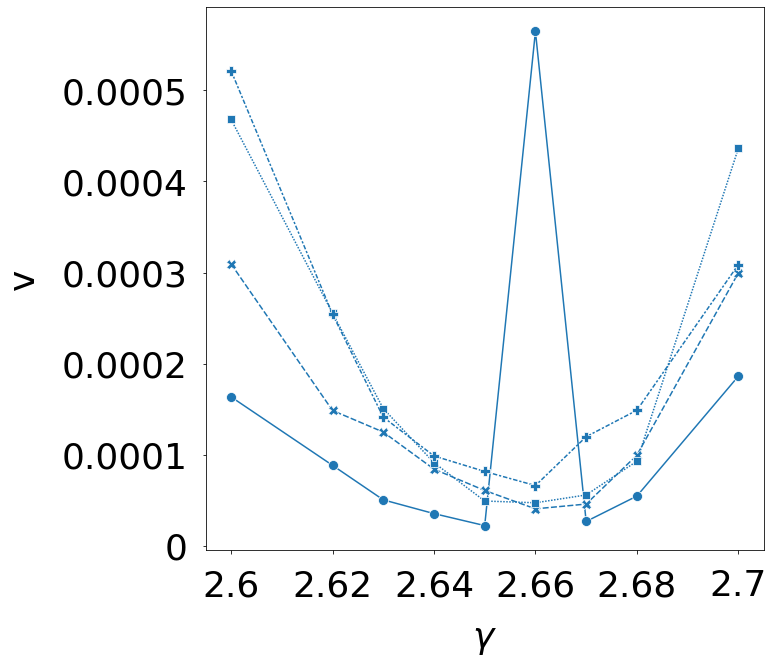
\includegraphics[height=\textwidth]{images/var_manna}
					\caption{Дисперсия}
				\end{subfigure}
				\hspace{5mm}
				\begin{subfigure}[t]{0.27\textwidth}
					\centering
					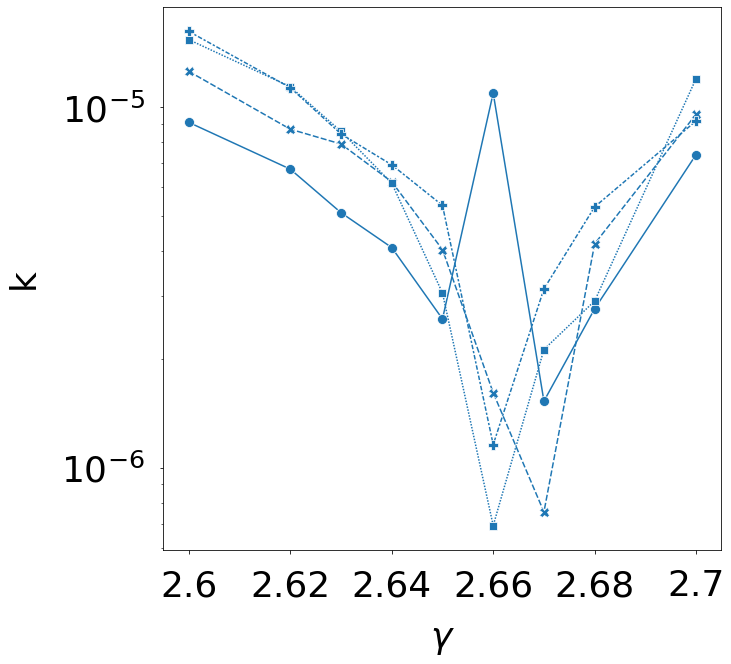
\includegraphics[height=\textwidth]{images/k_manna}
					\caption{Абсолютное значение коэффициента регрессирующей прямой}
				\end{subfigure}
				\hspace{0mm}
				\begin{subfigure}[t]{0.27\textwidth}
					\centering
					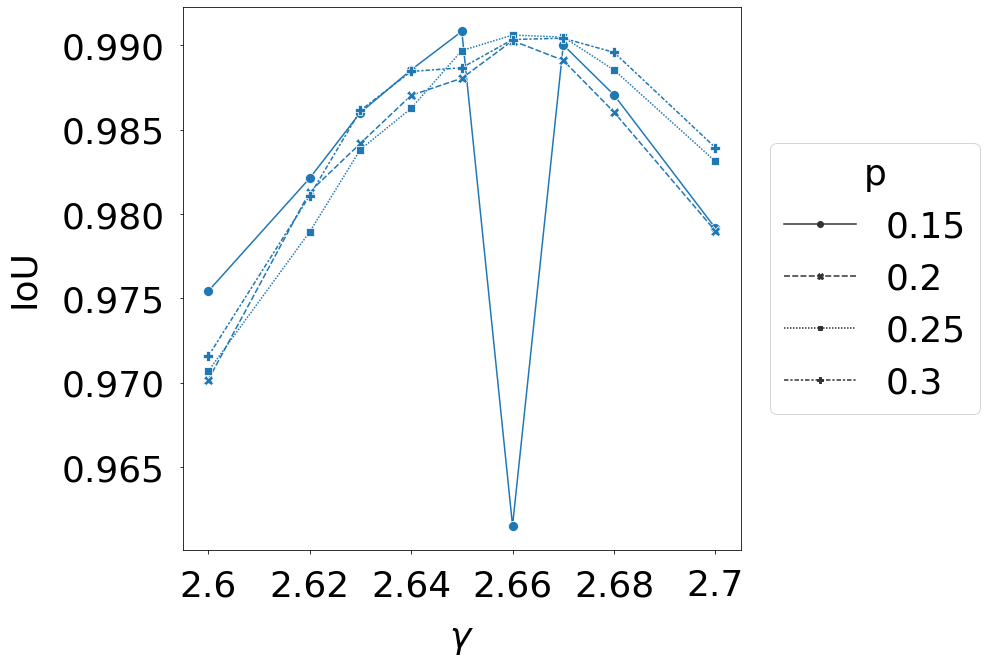
\includegraphics[height=\textwidth]{images/IoU_manna}
					\caption{IoU}
				\end{subfigure}
				\caption*{Метрики качества шкалирования в модели Манна в зависимости от параметра $\gamma$}\label{pic:manna_scaling_metrics}
			\end{figure}
		\end{onlyenv}
	\end{frame}
\end{document}
